\chapter{Lab 3: Sequential Programming} \label{day3}

\section{Timer}

In this exercise one of the most useful and important tools of the \gls{fpga} gets used: the clock. This enables sequential programming which can be used to create sounds and much more as we will see in later exercises.

This module uses the 100\,Mhz clock of the \gls{fpga} and outputs a lower frequency. The new clock remains high for only one cycle of the original clock. Therefore the clock first needs to be enabled in the constraints file. Then we implement a simple counter to output a slower clock signal. This method is not exactly precise as the counter cannot count in rational numbers, but its fairly close and sufficient for most use cases. For frequencies much lower than the input clock this module can be assumed to be accurate.

Here, we modified the maximum value to which the counter counts and always add one to the counter. A different but equivalently effective approach is to add the frequency to the counter and always count to 100 $\cdot 10^{6}$ (which is given by the 100\,MHz of the clock).

\lstinputlisting[language=VHDL]{./L3/E1/src/project_3_1.vhd}

\lstinputlisting[language=VHDL]{./L3/E1/src/project_3_1_1.vhd}

\section{Instantiating a netlist file}

In this exercise we use a given netlist file and instantiate it in our project to display a 14-bit binary number as a 4-digit decimal number on the four digit seven-segment display of the \gls{fpga}. 

\lstinputlisting[language=VHDL]{./L3/E2/src/project_3_2.vhd}

Additionally we used the given display.dcp display\_wrapper.vhd entity:

\lstinputlisting[language=VHDL]{./L3/E2/src/display_wrapper.vhd}

\section{Time counter}

Here, we programmed a counter that overflows implicitly and displays a new number every 0.5\,s on the four digit display of the \gls{fpga}. 

\begin{figure}[h]
	\centering
	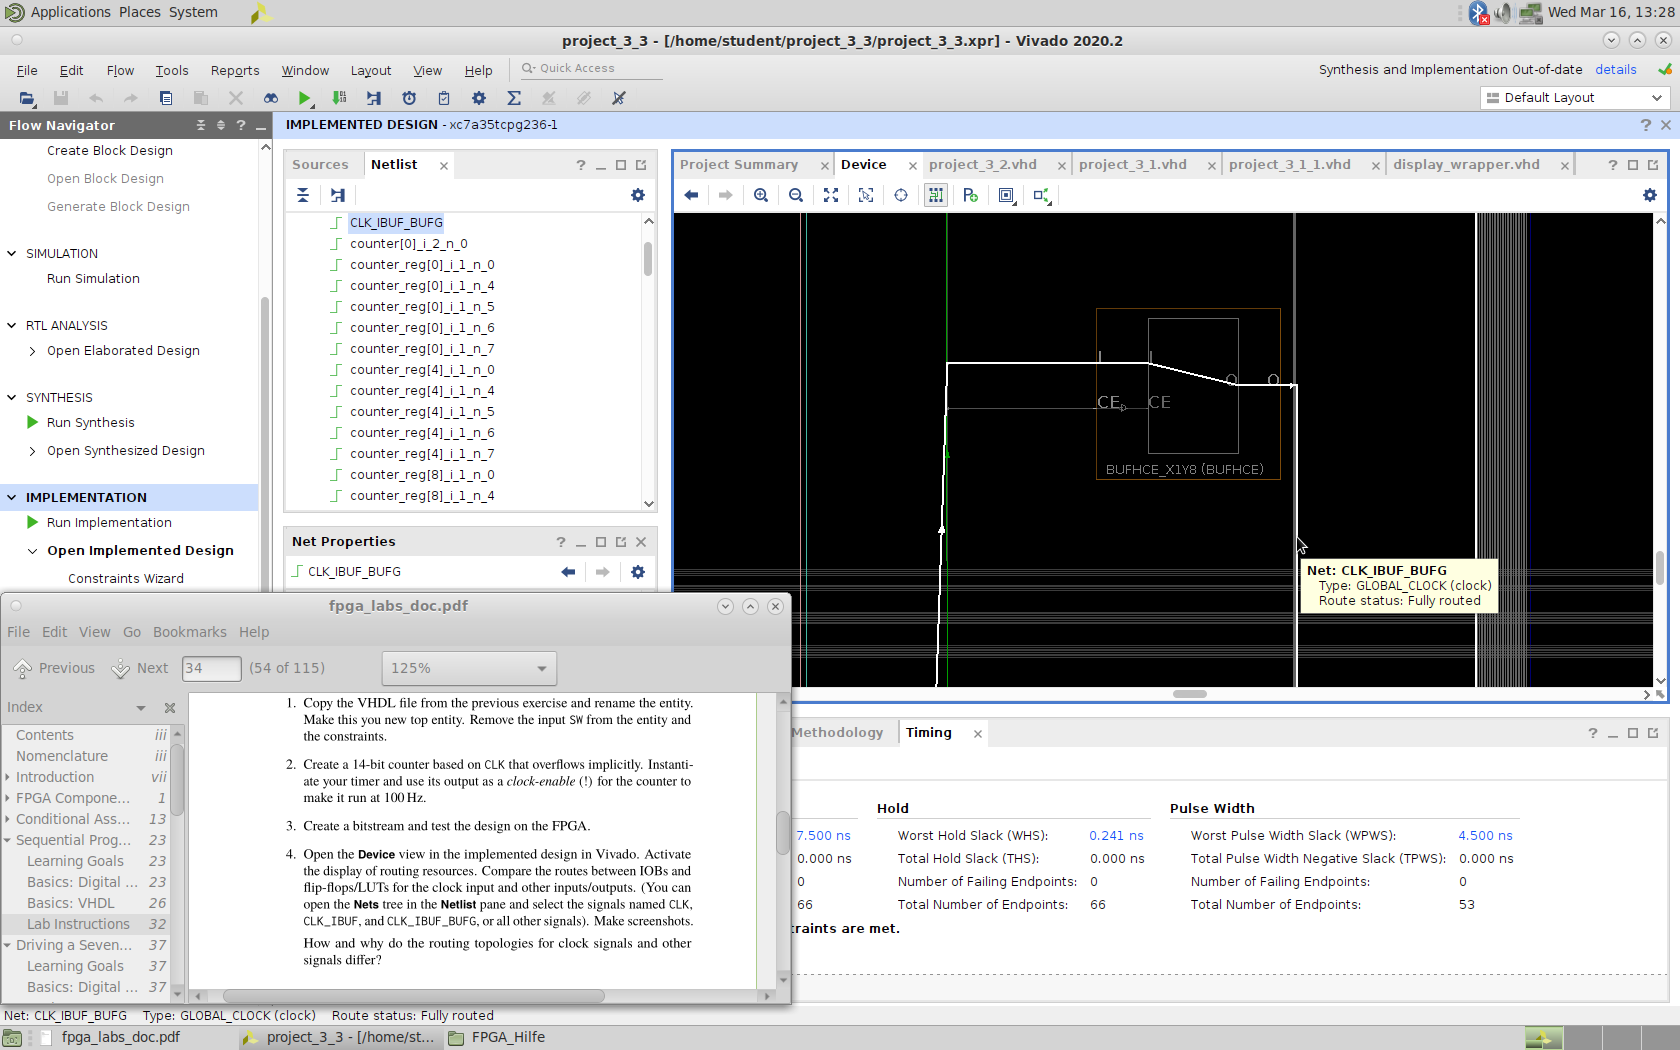
\includegraphics[width=.6\linewidth]{./L3/E3/BUFHCE.png}
	\caption{This clock signal is distributed via these centrally positioned buffer units on the \gls{fpga}.} 
	\label{fig: clock  e_3_3_1}
\end{figure}

\begin{figure}[h]
	\centering
	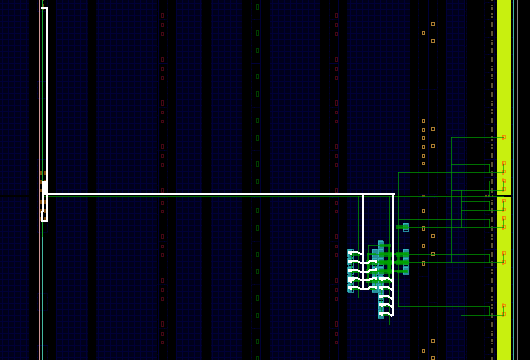
\includegraphics[width=.8\linewidth]{./L3/E3/CLK.png}
	\caption{The distribution of the clock signal. The clock signal is distributed over the central unit on the \gls{fpga} shown in fig. \ref*{fig: clock  e_3_3_1} and in this picture on the top left corner of the image. This design ensures that all the clock sensitive components (like Flip-Flops) of the circuit get almost the same clock signal to be in sync.}
	\label{fig: clock routing e_3_3_1}
\end{figure}

%\lstinputlisting[language=VHDL]{./L3/E3/src/project_3_1_1.vhd}

%\lstinputlisting[language=VHDL]{./L3/E3/src/project_3_1_1.vhd}

%\lstinputlisting[language=VHDL]{./L3/E3/src/project_3_1.vhd}

\lstinputlisting[language=VHDL]{./L3/E3/src/project_3_3.vhd}

The clock signal differs from other signal due to the required almost synchronous distribution. Therefore the \gls{fpga} has multiple central distribution units that ensure exactly this as can be seen in fig. \ref{fig: clock routing e_3_3_1}. Otherwise sequential programming cannot work correctly as intended.

Other circuits that do not require a clock signal can be routed with other priorities in mind. That could be to save space on the \gls{fpga} or to maximize throughput. 

\section{Debouncing}

The integrated buttons on the board of the \gls{fpga} have to be debounced in order to be used as an input. As the button bounces up and down multiple times after being pressed only once the ``button-pressed''-status has to be checked with a much lower frequency than the 100\,MHz clock. When pressing the button 20 times and checking the status with the 100\,MHz clock we found that much more than 20 presses were counted. To fix the issue, we used a 100\,Hz clock for checking if the button was pressed. That fixed the issue of multiple button presses being counted. Additionally we checked if the button has been pressed in the previous clock cycle of the 100\,Hz clock to eliminate any remaining errors. Checking the program with 50 button presses there were no more errors.

\lstinputlisting[language=VHDL]{./L3/E4/src/edge_detector.vhd}

\lstinputlisting[language=VHDL]{./L3/E4/src/project_3_4.vhd}

